\documentclass[conference]{IEEEtran}

\usepackage{amsmath,amssymb}
\usepackage{booktabs}
\usepackage{graphicx}
\usepackage{multirow}
\usepackage{url}

\begin{document}

\title{Graph-VerbalTS: Text-Conditioned Multivariate Time-Series Generation with Variable Dependency Graphs}

\author{
\IEEEauthorblockN{Anonymous Authors}
\IEEEauthorblockA{Anonymous Institution}
}

\maketitle

\begin{abstract}
Text-conditioned time-series generation aims to synthesize samples that satisfy natural-language descriptions. Existing methods such as VerbalTS condition generation on language but leave cross-variable structure implicit. In multivariate monitoring, this omission can produce individually plausible channels whose co-movements are inconsistent: coupled metrics may drift independently, anomaly signatures may fragment across subsystems, and the generated joint distribution may deviate from real system behavior. We propose Graph-VerbalTS, which injects a training-set Pearson dependency graph into the diffusion hidden representation and uses a lightweight GNN for variable-wise message passing during denoising. This supplies an explicit structural prior while preserving the original text-conditioning objective. We further introduce SMD-NL, aligning server-monitoring windows, window-level semantic metadata, and controlled natural-language descriptions. Across five random seeds, Graph-VerbalTS reduces FID from 6.4727 to 5.0756 and JFTSD from 7.1679 to 5.7076, with the improvement directionally consistent on every seed (paired Cohen's $d_z\approx1.2$--$1.3$; two-sided Wilcoxon $p=0.0625$), and an adapted external text-to-series baseline (T2S) trails by over $3\times$ on both distributional metrics. A metadata-conditioned baseline narrows the gap but requires subsystem labels at inference time. Identity- and random-graph ablations show that the gain is not explained by extra GNN layers or arbitrary connectivity, highlighting meaningful dependency modeling as the central contribution.
\end{abstract}

\begin{IEEEkeywords}
time-series generation, text-conditioned generation, diffusion models, graph neural networks, AIOps
\end{IEEEkeywords}

\section{Introduction}

Multivariate time series are common in server monitoring, industrial control, finance, and healthcare. They contain both temporal dynamics and dependencies among variables. In server monitoring, CPU utilization, load, memory usage, disk activities, network traffic, and connection states jointly characterize machine status. Generating sequences that follow temporal dynamics and satisfy user-provided semantic descriptions is therefore useful for data augmentation, anomaly-scenario simulation, and system-behavior analysis in intelligent operations.

Diffusion models provide strong distribution modeling for time-series generation, and language enables flexible control. VerbalTS~\cite{gu2025verbalts} shows that natural language is richer than structured metadata, but text conditioning and temporal modeling alone leave multivariate dependence implicit. This is consequential in server monitoring: load should co-vary with CPU metrics, disk reads with disk writes, and subsystem anomalies may appear jointly. Without explicit relational modeling, a generator can match each variable marginally yet combine them into physically or operationally inconsistent windows, weakening joint-distribution fidelity and the usefulness of generated scenarios.

To address this issue, we propose Graph-VerbalTS. The key idea is to introduce a fixed variable dependency graph into the text-conditioned diffusion generation framework of VerbalTS and to perform variable-wise message passing in the diffusion hidden representation. Instead of propagating graph information on raw inputs or post-processing generated outputs, we insert a graph module after multi-scale patch embedding and before residual diffusion layers. The variable dependency graph is computed from Pearson correlations on the training set and kept fixed during model training.

We further construct SMD-NL, a text-conditioned multivariate time-series dataset based on the Server Machine Dataset (SMD). We select 10 representative server-monitoring metrics, convert time-point anomaly labels into window-level semantic metadata, and use ChatTS to generate natural-language descriptions that are semantically consistent with the metadata while still allowing linguistic variation.

The main contributions are as follows:
\begin{itemize}
    \item \textbf{Dataset contribution:} We construct SMD-NL, aligning 10-variable server-monitoring windows, anomaly-derived metadata, and controlled natural-language descriptions.
    \item \textbf{Method contribution:} We propose Graph-VerbalTS, which injects a training-set Pearson graph into VerbalTS hidden denoising representations through a lightweight GNN, making cross-variable structure explicit.
    \item \textbf{Empirical contribution:} Five-seed comparisons with paired effect sizes, identity/random-graph and metadata-conditioning ablations, and an external T2S baseline show that meaningful dependency structure improves FID and JFTSD without sacrificing text--time-series alignment.
\end{itemize}

\section{Related Work}

\subsection{Time-Series Generation}

Time-series generation learns the distribution of real sequences and synthesizes samples with similar statistics and temporal patterns. Earlier methods rely on autoregressive or latent-variable assumptions, while deep generative models use adversarial or variational objectives. TimeGAN~\cite{yoon2019timegan}, which combines supervised temporal dynamics with adversarial learning, is representative. DoppelGANger~\cite{lin2020doppelganger} studies sharing networked time-series data with GANs, and TTS-GAN~\cite{li2022ttsgan} introduces a transformer-based adversarial generator for time series. Such models can generate realistic samples, but training stability, mode coverage, and conditional control remain challenging.

Diffusion models have achieved strong results in image, speech, and sequence generation. Early diffusion modeling connects generation with nonequilibrium thermodynamics~\cite{sohl2015nonequilibrium}, while score-based generative modeling estimates data-score functions for sampling~\cite{song2019score}. DDPM~\cite{ho2020ddpm} learns data distributions through progressive noising and denoising, and score-based SDEs provide a continuous-time view of the same family of models~\cite{song2021sde}. For time series, CSDI~\cite{tashiro2021csdi} applies conditional score-based diffusion to imputation, while TimeGrad~\cite{rasul2021timegrad} and TSDiff~\cite{kollovieh2023tsdiff} study diffusion or score-based probabilistic forecasting. Unlike image generation, multivariate time-series generation must handle temporal continuity, cross-variable dependencies, and task conditions; marginal variable distributions alone are often insufficient.

\subsection{Text-Conditioned Time-Series Generation}

Text-conditioned generation uses natural language to specify target samples. Traditional conditional time-series generation relies on labels, timestamps, statistical attributes, or structured metadata, whose expressiveness is limited. Recent work increasingly aligns time series with language models: LLMTime~\cite{gruver2023llmtime} studies zero-shot forecasting with language models, Time-LLM~\cite{jin2024timellm} transfers language-model capabilities to forecasting, and ChatTS~\cite{xie2025chatts} aligns time series with language models for understanding and reasoning.

VerbalTS~\cite{gu2025verbalts} further proposes a unified framework for generating time series from text and shows that natural-language descriptions provide richer conditions than structured metadata. T2S~\cite{ge2025t2s} trains a domain-agnostic text-to-series diffusion model with a length-adaptive VAE, but generates univariate series and offers no mechanism for variable-dependency conditioning. Unlike forecasting or understanding, text-conditioned generation requires the model to synthesize numerical sequences from language descriptions, which means that textual semantics, temporal dynamics, and data distributions must be jointly aligned. However, VerbalTS mainly focuses on mapping textual semantics to time-series shapes and does not explicitly model variable dependencies in multivariate systems. This paper extends VerbalTS by introducing variable dependency graphs so that generation is conditioned on both textual semantics and structural priors.

\subsection{Time-Series and Language Alignment}

Time-series and language alignment is the foundation of text-conditioned generation. Existing studies either convert time series into tokens or descriptions for language models, or align continuous time-series and text representations. ChatTS~\cite{xie2025chatts} emphasizes high-quality time-series--text pairs and uses synthetic data with attribute descriptions. We do not train a new time-series language model; instead, we use ChatTS as a controlled annotation tool to verbalize deterministic window-level metadata. This keeps text conditions natural while preserving consistency with anomaly labels and subsystem states.

\subsection{Graph Neural Networks for Multivariate Time Series}

Graph neural networks model relations in non-Euclidean data. GCN~\cite{kipf2017gcn} aggregates neighbors with normalized adjacency matrices, and GAT~\cite{velickovic2018gat} learns attention-based neighbor weights. For multivariate time series, variables, sensors, or spatial locations can be graph nodes, with correlations, physical connections, or topology as edges. STGCN~\cite{yu2018stgcn}, Graph WaveNet~\cite{wu2019graphwavenet}, and GMAN~\cite{zheng2020gman} show the value of graph structure in spatio-temporal modeling. MTGNN~\cite{wu2020mtgnn} further learns graph structures for multivariate forecasting when explicit topology is unavailable.

Existing graph-based time-series studies mainly focus on forecasting, classification, or anomaly detection. OmniAnomaly~\cite{su2019omnianomaly}, for example, targets multivariate time-series anomaly detection and provides the SMD used here, while GDN~\cite{deng2021gdn} applies graph neural networks to anomaly detection in multivariate time series. In contrast, we study text-conditioned generation: given a natural-language description, the model must generate a multivariate sequence matching the semantic condition. The task requires not only plausible individual variables but also credible cross-variable joint behavior.

\section{SMD-NL Dataset Construction}

Text-conditioned time-series generation requires paired natural-language conditions and numerical sequences, but such pairs are scarce in server-monitoring scenarios. Existing AIOps datasets usually provide numerical monitoring signals and labels rather than language. We therefore construct SMD-NL to turn a widely used multivariate server-monitoring benchmark into a controlled text-conditioned generation dataset.

\subsection{Raw Data and Variable Selection}

SMD-NL is constructed from SMD introduced by OmniAnomaly~\cite{su2019omnianomaly}. SMD contains real monitoring metrics with time-point anomaly labels, covers interacting compute, memory, disk, and network subsystems, and enables labels to be converted into window-level semantic metadata without relying on costly manually written operator reports.

The original SMD contains 38 metrics. Directly using all variables would increase modeling difficulty and introduce substantial redundancy for a first text-conditioned generation benchmark. We select 10 representative metrics, grouped by subsystem in Table~\ref{tab:selected_metrics}, retaining the cross-variable structure needed for dependency-aware generation.

\begin{table}[t]
\centering
\caption{Selected server-monitoring metrics in SMD-NL.}
\label{tab:selected_metrics}
\begin{tabular}{llc}
\toprule
Subsystem & Metric & Original index \\
\midrule
Compute & \texttt{cpu\_r} & 0 \\
Compute & \texttt{load\_1} & 1 \\
Memory & \texttt{mem\_u\_e} & 6 \\
Disk & \texttt{disk\_r} & 9 \\
Disk & \texttt{disk\_u} & 12 \\
Disk & \texttt{disk\_w} & 13 \\
Network & \texttt{eth1\_pi} & 20 \\
Network & \texttt{eth1\_po} & 21 \\
Network & \texttt{tcp\_use} & 23 \\
Network & \texttt{curr\_estab} & 25 \\
\bottomrule
\end{tabular}
\end{table}

\subsection{Windowing and Data Splits}

We segment sequences with a sliding window of length 240 and stride 120. Adjacent windows overlap by 50\%, increasing sample count while preserving local continuity. Each window is a $240\times10$ multivariate sample and serves as the unit for metadata construction, annotation, training, and evaluation. Anomaly labels are used only to construct metadata and text conditions, not as prediction targets. Samples are split into training, validation, and test sets at a ratio of $7:1:2$, with boundaries handled at the original-sequence level to prevent leakage from overlapping windows. Statistics are shown in Table~\ref{tab:dataset_stats}.

\begin{table}[t]
\centering
\caption{SMD-NL statistics.}
\label{tab:dataset_stats}
\begin{tabular}{lccc}
\toprule
Split & Windows & Length & Variables \\
\midrule
Train & 4104 & 240 & 10 \\
Validation & 587 & 240 & 10 \\
Test & 1173 & 240 & 10 \\
\bottomrule
\end{tabular}
\end{table}

\subsection{Window-Level Metadata}

We convert time-point anomaly labels into window-level structured metadata. The variables are grouped into compute $\{0,1\}$, memory $\{6\}$, disk $\{9,12,13\}$, and network $\{20,21,23,25\}$ subsystems, with an additional global state. For each window and subsystem, we compute anomaly ratio $r$ and assign state $s$ as
\begin{equation}
s=
\begin{cases}
\text{normal}, & r=0\%,\\
\text{mildly abnormal}, & 0\%<r\leq10\%,\\
\text{severely abnormal}, & r>10\%.
\end{cases}
\label{eq:state}
\end{equation}
The same rule determines the global state. Compared with binary labels, the three-level representation describes abnormality more naturally and is easier to verbalize.

\subsection{Natural-Language Description Generation}

After obtaining metadata, we use ChatTS-14B based on Qwen2.5-14B to verbalize structured states. The model is not allowed to infer labels freely from curves. Instead, \texttt{test\_label} and \texttt{interpretation\_label} are used to construct a time-step--variable anomaly matrix and deterministic global/subsystem states, which serve as the primary semantic constraints.

The annotation input contains the 10-variable window and its global, compute, memory, disk, and network states. ChatTS uses curves only for observable patterns and is instructed not to invent exact values, timestamps, root causes, failure types, diagnoses, or future trends. For each window, it produces three 35--70 word descriptions: a concise operating-state summary, a subsystem-oriented description, and a temporal-pattern-oriented description. Training randomly samples one description; validation and testing use a fixed description. Table~\ref{tab:annotation} summarizes the protocol.

\begin{table*}[t]
\centering
\caption{Core constraints in the ChatTS annotation protocol.}
\label{tab:annotation}
\begin{tabular}{p{0.19\textwidth}p{0.73\textwidth}}
\toprule
Item & Constraint \\
\midrule
Main semantic evidence & Use global, compute, memory, disk, and network states as primary semantic constraints. \\
Use of curves & Describe only observable trends, fluctuations, spikes, stable intervals, and co-variation patterns. \\
Forbidden content & Do not invent exact values, timestamps, root causes, device failures, diagnoses, or future outcomes. \\
Output form & Generate three 35--70 word English descriptions per window with consistent semantics and varied styles. \\
\bottomrule
\end{tabular}
\end{table*}

\subsection{Dataset Characteristics}

SMD-NL aligns each monitoring window with structured metadata and natural-language descriptions, preserves subsystem structure across compute, memory, disk, and network variables, and provides multiple semantically equivalent descriptions per window. Deterministic metadata plus controlled ChatTS annotation favors semantic consistency and reproducibility.

\section{Method}

\subsection{Problem Definition}

Given a natural-language description $c$, text-conditioned multivariate time-series generation learns to synthesize $x_0\in\mathbb{R}^{L\times V}$, where $L$ is sequence length and $V$ is the number of variables. In SMD-NL, $L=240$ and $V=10$. The sample should match $c$ while preserving realistic temporal variation and cross-variable dependence.

\subsection{VerbalTS Backbone}

We use VerbalTS~\cite{gu2025verbalts} as the backbone. It encodes text through a pretrained language encoder and maps noisy multivariate sequences into a diffusion hidden representation through multi-scale patch embedding. Residual diffusion layers then predict noise at each diffusion step. This design models temporal structure and text conditions, but cross-variable relationships remain implicit in the shared hidden representation.

Graph-VerbalTS keeps the text-conditioning mechanism, sampling process, and training objective unchanged and adds only a variable-graph module to the hidden representation. This isolates dependency modeling as the architectural difference.

\begin{figure*}[t]
    \centering
    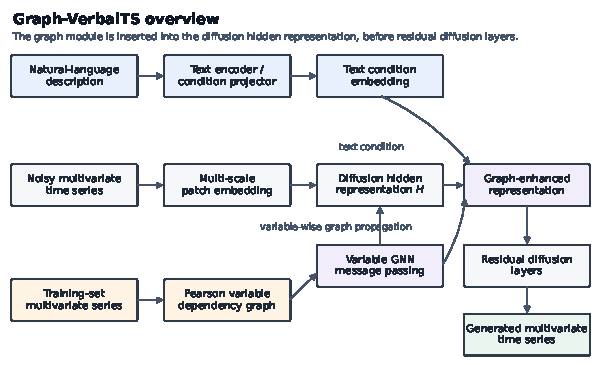
\includegraphics[width=0.78\textwidth]{figures/graph_verbalts_overview.pdf}
    \caption{Overview of Graph-VerbalTS. Natural-language descriptions are encoded as text conditions, while noisy multivariate time series are mapped into diffusion hidden representations through multi-scale patch embedding. A training-set Pearson graph and lightweight GNN provide variable-wise message passing before residual diffusion layers.}
    \label{fig:overview}
\end{figure*}

\subsection{Variable Dependency Graph Construction}

We construct a fixed Pearson dependency graph from training data to avoid test leakage. The training tensor is reshaped from $N\times L\times V$ to $(N\cdot L)\times V$, and correlations are computed between variables. Absolute correlations are used as edge strengths so both positive and negative dependencies contribute. For each variable, the top-$k$ neighbors are retained, with $k=3$ in the main experiments. We add self-loops, symmetrize the adjacency matrix, and apply GCN normalization:
\begin{equation}
\tilde{A}=D^{-\frac{1}{2}}AD^{-\frac{1}{2}},
\label{eq:normalization}
\end{equation}
where $A$ is the adjacency after adding self-loops and $D$ is its degree matrix. The resulting $\tilde{A}$ is a fixed buffer rather than a trainable parameter. Identity and random graphs are used as ablation variants.

\subsection{Graph-Enhanced Diffusion Hidden Representation}

Let $H\in\mathbb{R}^{B\times C\times V\times L_p}$ be the hidden representation after multi-scale patch embedding, where $B$ is batch size, $C$ is hidden channels, $V$ is variables, and $L_p$ is temporal patch dimension. Graph-VerbalTS first permutes it to
\begin{equation}
H'\in\mathbb{R}^{B\times L_p\times V\times C},
\label{eq:permutation}
\end{equation}
and performs graph convolution along the variable dimension:
\begin{equation}
Z=\sigma(\tilde{A}H'W),
\label{eq:gcn}
\end{equation}
where $W$ is a trainable projection and $\sigma$ is a nonlinear activation. The output is converted back to $\mathbb{R}^{B\times C\times V\times L_p}$ and sent to subsequent residual diffusion layers. We use a residual connection:
\begin{equation}
H_{\mathrm{graph}}=H+\operatorname{GNN}(H,\tilde{A}).
\label{eq:residual}
\end{equation}
The graph module performs message passing only along variables and does not alter temporal-patch ordering, preserving VerbalTS temporal modeling while introducing cross-variable interaction.

\begin{figure*}[t]
    \centering
    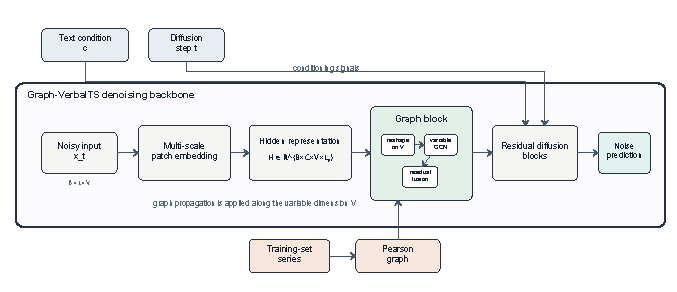
\includegraphics[width=0.88\textwidth]{figures/graph_verbalts_backbone.pdf}
    \caption{Backbone architecture of Graph-VerbalTS. Multi-scale patch embedding maps the noisy input into a hidden representation. The graph block applies variable-wise message passing with the training-set Pearson graph before residual diffusion blocks predict noise under text and diffusion-step conditioning.}
    \label{fig:backbone}
\end{figure*}

\subsection{Training Objective}

Graph-VerbalTS follows the VerbalTS diffusion noise-prediction objective. Given real sequence $x_0$, text condition $c$, diffusion step $t$, and noise $\epsilon$, the model predicts the noise added to $x_t$:
\begin{equation}
\mathcal{L}=\mathbb{E}_{x_0,c,t,\epsilon}
\left[\left\|\epsilon-\epsilon_{\theta}(x_t,t,c,\tilde{A})\right\|_2^2\right].
\label{eq:loss}
\end{equation}
When the graph module is disabled, the model reduces to VerbalTS.

\section{Experiments}

\subsection{Experimental Setup}

We evaluate on SMD-NL. During training one of three descriptions is sampled at random; validation and testing use a fixed description. We compare VerbalTS, Graph-VerbalTS, an identity graph retaining only self-loops, and a random graph with the same edge density and normalization pipeline as the Pearson graph. As an external reference we further include T2S~\cite{ge2025t2s}, a recent text-to-series diffusion model.

All variants use the same splits, text encoder, and diffusion backbone. The diffusion network has 3 residual diffusion layers, hidden channel size 64, diffusion embedding dimension 128, 4 attention heads, and 50 diffusion steps. Multi-scale patch settings are \texttt{multipatch\_num=3}, base patch length 1, and multiplier 3. The GNN has 2 graph-convolution layers, hidden dimension 64, dropout 0.1, and residual connections. Graph-VerbalTS uses top-$k=3$ Pearson neighbors.

The main experiments use 5 random seeds (seeds 1, 7, 42, 100, and 123) and train for 30 epochs with batch size 16, learning rate $5\times10^{-5}$, gradient clipping 1.0, and validation every 10 epochs. All methods share the same hyperparameters and seed set; the identity-graph ablation uses the first three seeds. We additionally compare a \emph{metadata-conditioned} variant of VerbalTS that replaces the natural-language description with the five structured subsystem states used in SMD-NL, encoded by a lightweight attribute embedding; this isolates the value of language conditioning under the identical backbone.

For the external baseline, we adapt T2S to SMD-NL as follows: the length-adaptive VAE is retrained on the ten-channel windows with per-variable normalization, the DiT denoiser is conditioned on the same frozen text embeddings used by our variants, and generation follows the identical protocol of ten samples per window with the window-wise median. T2S is fully retrained for each of the five seeds. We use the authors' default flow-matching sampler; no graph module or multivariate conditioning is available in the original design.

\subsection{Evaluation Metrics}

We use FID, JFTSD, and CTTP following the VerbalTS evaluation protocol, with the same frozen text and time-series encoders across variants. FID measures the Fr\'echet distance between generated and real time-series embedding distributions. JFTSD measures the Fr\'echet distance between generated and real joint text--time-series embedding distributions. CTTP is computed as the mean over test windows of the dot product between the frozen CTTP encoder embedding of the generated window and that of its paired text description; because these embeddings are not $\ell_2$-normalized, values are on the order of 10, and higher values indicate stronger condition matching. They evaluate time-series distribution quality, joint semantic distribution, and condition matching, respectively.

\subsection{Main Results}

Table~\ref{tab:main_results} reports mean and standard deviation over 5 random seeds (3 for the identity-graph ablation). Graph-VerbalTS achieves the best mean FID and JFTSD. Relative to VerbalTS, it reduces FID from 6.4727 to 5.0756 (21.6\%) and JFTSD from 7.1679 to 5.7076 (20.4\%), indicating better time-series and joint text--time-series distributions. The adapted T2S baseline trails by a wide margin ($3.3\times$ our FID, $3.3\times$ our JFTSD, and worse than text-only VerbalTS by $2.6\times$), confirming that a univariate text-to-series design transfers poorly to multivariate monitoring data.

\begin{table*}[t]
\centering
\caption{Main results on SMD-NL. Lower FID and JFTSD are better, while higher CTTP is better. Values are mean $\pm$ standard deviation over 5 random seeds, except the identity-graph ablation (3 seeds). T2S is an external baseline adapted to multivariate windows.}
\label{tab:main_results}
\begin{tabular}{lccc}
\toprule
Method & FID $\downarrow$ & JFTSD $\downarrow$ & CTTP $\uparrow$ \\
\midrule
T2S (external) & $16.9203\pm2.2711$ & $18.9799\pm2.2337$ & $11.7273\pm0.1435$ \\
VerbalTS & $6.4727\pm1.4677$ & $7.1679\pm1.4228$ & $10.8251\pm0.1409$ \\
Metadata-conditioned VerbalTS & $5.3065\pm0.8354$ & $5.9404\pm0.7820$ & $10.6559\pm0.1341$ \\
Identity graph ablation & $6.1086\pm0.4039$ & $6.7109\pm0.3851$ & $10.8385\pm0.0658$ \\
Random graph ablation & $5.5003\pm1.0918$ & $6.1265\pm1.0535$ & $10.7874\pm0.1163$ \\
Graph-VerbalTS & $\mathbf{5.0756\pm0.8803}$ & $\mathbf{5.7076\pm0.8416}$ & $10.7572\pm0.0852$ \\
\bottomrule
\end{tabular}
\end{table*}

The comparison clarifies the cost of leaving multivariate correlation implicit: VerbalTS can generate plausible per-variable trajectories, yet its higher joint-distribution distances indicate less faithful variable combinations. The identity graph retains GNN layers but blocks cross-variable messages, yielding limited gains. The random graph permits messages but remains worse than the Pearson graph. Thus, improvement is attributable neither to parameter count nor arbitrary connectivity, but to data-supported dependency structure. CTTP remains comparable across all variants (all means lie within 0.19, comparable to within-seed variability), indicating that the structural prior does not trade off text--time-series matching. The metadata-conditioned variant is the strongest non-graph baseline: feeding the five structured subsystem states to the same backbone already improves upon text-only conditioning, showing that the benefit of conditioning stems largely from supplying system-state information in any form. However, it requires these labels at inference time, which in practice must come from an external anomaly-detection module, whereas our variant conditions on natural language available from operators and derives the dependency graph from training data alone. Graph-VerbalTS still attains the best FID and JFTSD, so explicit Pearson structure recovers and slightly exceeds what structured labels provide, without additional inference-time instrumentation.

T2S shows the opposite pattern on CTTP: it attains the highest condition-matching score (11.73) while failing on both distributional metrics. Because T2S is conditioned directly on the frozen CTTP text embeddings, its samples can align closely with the text-embedding direction without reproducing the multivariate data distribution, which the FID and JFTSD penalize. This dissociation indicates that condition matching alone can be satisfied by embedding-space proximity and motivates reporting distributional and semantic metrics jointly. For reference, the real-test CTTP self-similarity is 12.16, so T2S approaches the reference on this metric while remaining far from the real data distribution by FID and JFTSD.

\subsection{Graph Structure Ablation and Statistical Analysis}

The identity and random graph ablations examine whether gains come merely from additional GNN parameters or arbitrary message passing. Graph-VerbalTS retains the best mean FID and JFTSD, and its standard deviations are lower than those of VerbalTS and the random-graph variant. To quantify within-seed consistency, we run paired seed-wise tests on the five common seeds. Graph-VerbalTS attains lower FID and JFTSD than VerbalTS on all five seeds, and lower than the random graph on all five seeds. The two-sided Wilcoxon signed-rank test reaches its minimum attainable $p$-value of $0.0625$ at $n=5$ for both FID and JFTSD against VerbalTS and against the random graph; paired $t$-tests yield $p=0.041$ (JFTSD) and $p=0.051$ (FID) against VerbalTS, and $p\approx0.054$--$0.055$ against the random graph. The corresponding paired effect sizes are Cohen's $d_z\approx1.2$--$1.3$, a large effect. Against the metadata-conditioned variant, differences on FID and JFTSD are small and not significant ($p\approx0.7$--$0.8$, $d_z\approx0.2$); the identity-graph ablation, run on three seeds, remains directionally consistent but below formal significance ($p=0.25$ at $n=3$). We therefore interpret the graph-structure results as consistent per-seed improvements with large paired effects and borderline formal significance at this sample size. Against T2S, the margin is far larger than the seed-level variability: Graph-VerbalTS attains lower FID and JFTSD on all five seeds, with mean gaps of $3.3\times$, so no formal test is needed to separate the two.

\subsection{Qualitative Analysis}

Figure~\ref{fig:graphs} visualizes the Pearson correlation matrix, Pearson graph, identity graph, and random graph. Training data contain structured dependency patterns among compute, disk, and network metrics. After top-$k$ filtering and normalization, the Pearson graph retains data-supported cross-variable connections; the identity graph contains only self-connections and the random graph lacks monitoring-consistent structure.

\begin{figure*}[t]
    \centering
    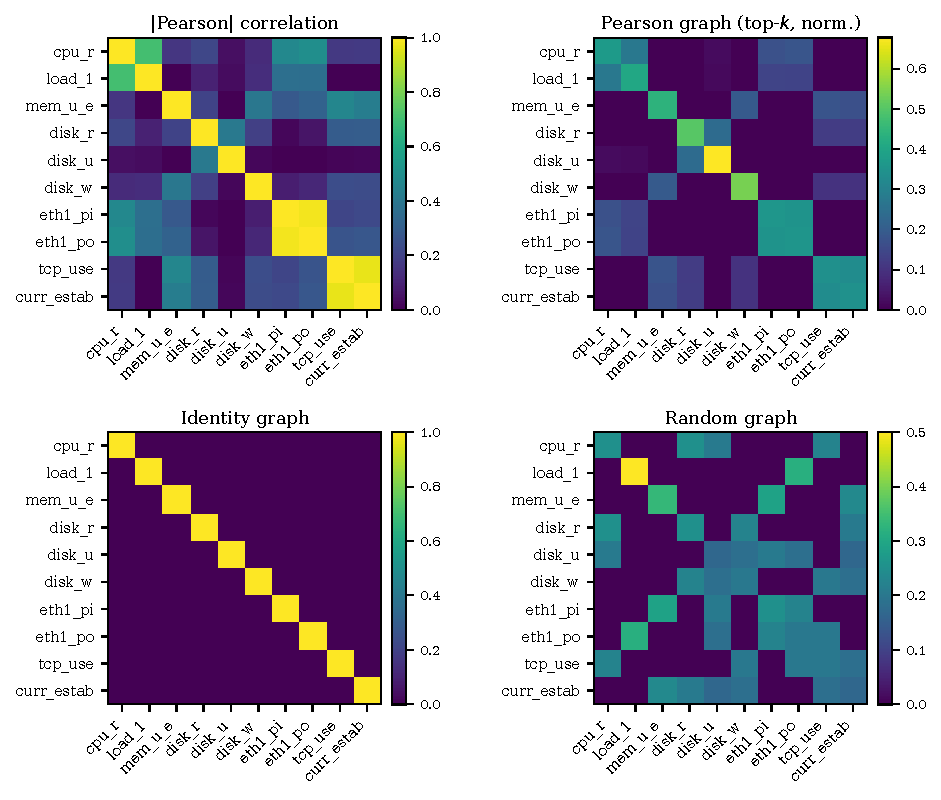
\includegraphics[width=0.92\textwidth]{figures/graph_heatmaps_latest.pdf}
    \caption{Graph structure visualization on SMD-NL. The Pearson graph retains dependency edges after top-$k$ filtering, self-loops, and GCN normalization; the identity graph keeps only self-connections; and the random graph introduces random cross-variable edges without interpretable structure. Axis abbreviations follow Table~\ref{tab:selected_metrics}.}
    \label{fig:graphs}
\end{figure*}

Figure~\ref{fig:samples} compares real sequences, VerbalTS generations, and Graph-VerbalTS generations on held-out test windows. The variables cover network, compute, load, and connection-related signals and complement the aggregate metrics in Table~\ref{tab:main_results}.

\begin{figure*}[t]
    \centering
    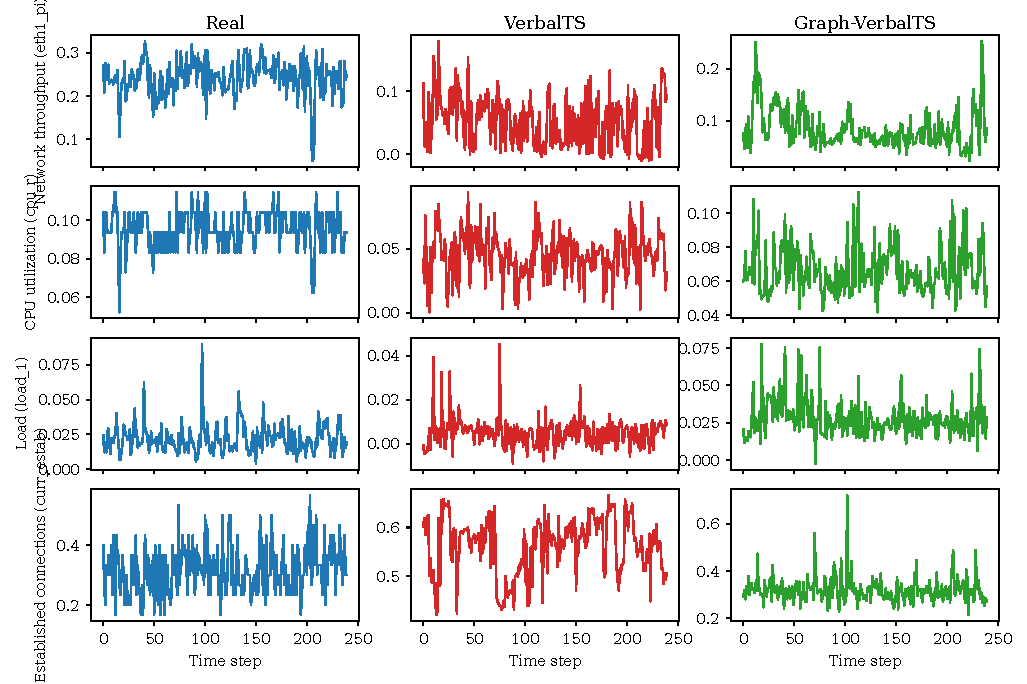
\includegraphics[width=0.92\textwidth]{figures/sample_comparison_latest.pdf}
    \caption{Curve comparison among real sequences, VerbalTS generations, and Graph-VerbalTS generations on held-out test windows. Rows show network-throughput, CPU-utilization, load, and connection-count variables.}
    \label{fig:samples}
\end{figure*}

\section{Discussion and Limitations}

Across repeated random seeds with paired seed-wise analysis, the results identify explicit dependency modeling as the empirical contribution. A text-conditioned denoiser without a relational mechanism must infer all cross-variable structure indirectly from shared hidden features. It may reproduce realistic marginal shapes while breaking co-movement, producing contradictory subsystem states, or dispersing a coherent multivariate anomaly across unrelated channels. The higher FID and JFTSD of VerbalTS quantify this loss of joint fidelity. Identity and random graphs further show that extra layers or message passing alone are insufficient; the useful signal is data-supported Pearson structure. The metadata-conditioned variant reinforces this reading: structured labels already help, yet matching the graph-augmented quality requires an external detector at inference time, while Graph-VerbalTS reaches the same operating point from text plus a training-data graph. Comparable CTTP confirms that the structural prior complements, rather than overrides, language conditioning.

There are several limitations and natural extensions. First, experiments are conducted on SMD-NL, and broader validation would further test generalization. Second, the graph is fixed and constructed from global Pearson correlations; dynamic or learned graphs may capture nonlinear, directional, sample-specific, or time-varying dependencies. Third, the current evaluation uses five random seeds (three for the identity-graph ablation); although paired differences are directionally consistent with large effect sizes and borderline Wilcoxon significance, evaluation with more seeds and across datasets would enable stronger statistical claims. Fourth, descriptions are generated by ChatTS from structured metadata; future work may incorporate real operator reports or human-in-the-loop annotation.

\section{Code and Data Availability}

SMD-NL is constructed from the public Server Machine Dataset~\cite{su2019omnianomaly}. The windowing, metadata construction, and annotation pipeline, together with the full training, evaluation, ablation code for Graph-VerbalTS, the metadata-conditioned variant, all graph-structure ablations, and our multivariate T2S adaptation, will be publicly released upon acceptance; an anonymized repository is provided to reviewers in the submission system.

\section{Conclusion}

This paper contributes a dependency-aware formulation of text-conditioned multivariate time-series generation. Graph-VerbalTS injects a training-set Pearson graph into the diffusion hidden representation, where a lightweight GNN coordinates variable-wise denoising without changing the original text and diffusion objectives. We also contribute SMD-NL, which aligns server-monitoring windows, window-level semantic metadata, and natural-language descriptions. Experiments across repeated random seeds and graph-structure ablations show why explicit structure matters: realistic individual channels can still form an inaccurate joint system state. Graph-VerbalTS improves FID and JFTSD by 21.6\% and 20.4\% with improvements on every seed and comparable CTTP, and clearly outperforms an adapted external text-to-series baseline, supporting meaningful dependency structure as a practical structural prior. Future work will study dynamic or learned graphs, broader domains, larger-scale statistical evaluation, and finer-grained text control.

\bibliographystyle{IEEEtran}
\bibliography{references}

\end{document}
